\chapter{今後の業務への貢献・活用}
\acrshort{sil2linuxmp}プロジェクトは2017年11月までに完結することが目標とされている。
プロジェクト2年目となる2016年度では、日立はこれまでと同様に\acrshort{sil2linuxmp}コミュニティへの働きかけを継続するとともに、
\acrshort{sil2linuxmp}プロジェクトで得た知見を社内の製品開発に還元していく活動を行う。
2016年度に実施すべき課題として以下の3つを設定する。
\begin{itemize}
  \item \acrshort{oss}・\acrshort{linux}システムの機能安全対応パイロット開発実施
  \item 機能安全対応\acrshort{linux}ディストリビューションの構築と提案
  \item \acrshort{sil2linuxmp}コミュニティへの継続的なコントリビューション
\end{itemize}
\section{\acrshort{oss}・\acrshort{linux}システムの機能安全対応パイロット開発実施}
\acrshort{sil2linuxmp}プロジェクトは特定のシステムに対して機能安全認証を与えることを目指すのではなく、
一般に\acrshort{oss}・\acrshort{linux}を使ったシステムで機能安全認証を達成するためのプロセスおよび方法論を確立することを意図している。
そのため、開発されたプロセスと方法論が現実の製品に即して適用できることの事例を残すことが、
将来\acrshort{sil2linuxmp}の成果によって\acrshort{oss}・\acrshort{linux}が\acrshort{sc}なシステムで使われるようになるために重要である。
特に、現在\acrshort{sil2linuxmp}で開発されている\acrshort{cr}
(\acrshort{iec61508}文書をRoute$3_S$: assessment of non-compliant developmentに基づいて
\acrshort{oss}・\acrshort{linux}システムに適用できるよう解釈し具体的な手段を対応させたもの)
の詳細や実現方法が不完全であると\acrshort{tuv}から指摘されている。
この問題の一因として、\acrshort{sil2linuxmp}プロジェクトにおいてターゲットとなるユースケースとシステム構成が定まっていないために、
具体的に何に対してどのようにプロセス・方法論を適用するのかがコミュニティ内で明確に共有されていないことが挙げられる。
\par
日立はグループ内で開発されている\acrshort{linux}ベースの\gls{adas}に機能安全認証を与えることを目標に
\acrshort{sil2linuxmp}で開発されたプロセスと方法論の適用を試みることで、
\acrshort{cr}の具体化と\acrshort{oss}・\acrshort{linux}の\acrshort{sil2}対応事例確立を目指す。
この活動はソースコード自体の開発よりも、開発プロセスのトレーサビリティと開発体制の健全性を確保すること、
および定められたプロセスが適切に実施されていることのエビデンスを体系的に蓄積することが中心となる。
特に、使用するソフトウェアの選定、アーキテクチャ設計、リスク分析など特定の個人の評価に依存しがちな
様々な判断事項について、その判断に至るまでの議論の経過と判断基準を全て記録することが必要となる。
これらの記録は第三者認証機関のレビューを受ける場において、自ら構築したシステムが正しく設計されていることを証明するための材料となる。
日立ではこのことを「基本と正道」と言う。
同様の概念が\href{http://www.slideshare.net/chika_nakazawa/ss-27726686}{サイボウズでは「公明正大」と言われている}。 \cite{cybozu}
\par
具体的には、\acrshort{sil2linuxmp}プロジェクトで定期的に行われている\gls{hazop}セッションを利用して日立\acrshort{adas}システムのハザード分析を行う。
\acrshort{hazop}はシステムの潜在危険因子を定量的かつ網羅的に抽出・評価するプロセスで、予め定められた役割と手法によるチームワークで進行する。
\acrshort{sil2linuxmp}コミュニティは\acrshort{irc}とwebベースのツールを活用して\acrshort{hazop}をオンラインで行う仕組みを構築しており、
これによって遠隔メンバの参加や議論内容の確実な保存と事後参照が可能となっている。
また\acrshort{db4sil2}(\ref{db4sil2sec}項)を利用して検証結果のエビデンスを保存することや、
ソフトウェア部品とツールの選定評価基準を定めた\acrshort{sil2linuxmp}ドキュメント\gls{atc}に基づいた評価、
および\acrshort{ogsn}を利用してその評価過程を可視化する活動を行う。
\section{機能安全対応\acrshort{linux}ディストリビューションの構築と提案}
\acrshort{sil2linuxmp}と関連して、日立製品の共通ソフトウェア基盤として使用されることを目的とした独自の\acrshort{linux}ディストリビューション開発が進行している。
これは特に\acrshort{sc}な産業・インフラ分野で10年単位の長期間にわたって稼動するシステムを意図したものであり、
将来的に\acrshort{sil2linuxmp}の成果を取り込むことで機能安全案件にも対応できるサービスを実現することが計画されている。
\par
\acrshort{linux}ディストリビューションが多くのユーザに使用してもらえるようになるためには、タイムリーなメンテナンスサポートを継続的に提供することが必須である。
一般的に使用されているディストリビューションは全てパッケージ管理システムを持っており、ユーザはこれによって必要なバグ修正やセキュリティ更新を簡単な手順で適用することができる。
このようなメンテナンスサポートがないと、ユーザが全ての\acrshort{oss}アップストリームを監視して適用すべき変更を自分自身で判断した上で適用評価まで行わなければならないことになり、
\acrshort{linux}システム上でのアプリケーション開発にとって非現実的な量の負担となる。
%\par
我々が手厚いメンテナンスサービスを利用できるのはディストリビュータに所属するその分野のエキスパートの貢献に負うところが大きく、それはある意味属人的なプロセスでもある。
\acrshort{iec61508}-3 7.8 Software modification の項目に「ソフトウェアの改変プロセスが適切に定義され透明性を持って運用されること」という旨の内容が語られている通り、
機能安全対応のディストリビューション開発においてはアップストリームの監視とバグ修正・セキュリティ更新の適用評価プロセスのトレーサビリティが確保されることが求められる。
独自に機能安全対応\acrshort{linux}ディストリビューションを構築するとなると、数ある\acrshort{oss}プロジェクトを属人的でないプロセスで監視するためには何らかの自動化対策が不可欠となる。
\par
\acrshort{sil2linuxmp}プロジェクトでは\pageref{scale}ページで述べたように検証プロセスを自動化するための様々なツール・技法が検討されている。
図\ref{QA_Tools}は品質管理ライフサイクルの各タスクで適用できる可能性のあるツール・技法の対応付けを示したものである。
これを機能安全対応ディストリビューションに拡張するためには、図\ref{QA_Tools}に加えて「アップストリームの監視と適用すべき変更の抽出」をシスティマティックに実施する仕組みの導入が必要となる(図\ref{safedist})。
\begin{figure}[ht]
  \centering
  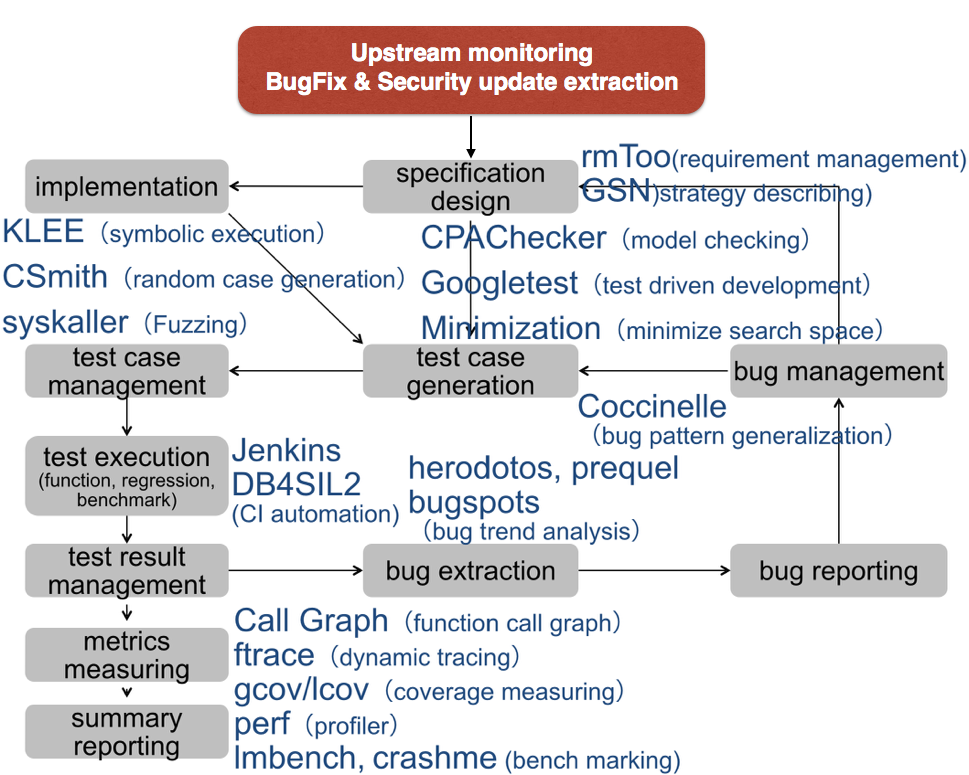
\includegraphics[width=\textwidth]{pic/safedist.eps}
  \caption{検証フレームワークの機能安全対応\acrshort{linux}ディストリビューションへの拡張}
  \label{safedist}
\end{figure}
\par
監視するべき\acrshort{oss}プロジェクトは多数存在するが、それらの開発基盤には事実上の世界標準であるバージョン管理システム\acrshort{git}が共通して使われている。
\acrshort{git}には全ての変更履歴がパッチとして記録されており、パッチにはそれぞれ変更の内容・意図・背景に関するコメントが付与されている。
アップストリームの監視と適用すべき変更の抽出を自動化するためには、\acrshort{git}パッチに含まれる情報を最大限利用する戦略が考えられる。
\pageref{presec}ページでは\acrshort{git}変更履歴に対してセマンティックパターンサーチを行うツール\acrshort{pre}を述べた。
\acrshort{pre}の戦略を拡張して、パッチコメントに対するセマンティックパターンサーチを行うことが出来れば
例えば特定のレベルのバグ修正やセキュリティ更新を効率よく抽出できる可能性がある。
その後の評価や適用判断は人の介在が必要であるものの、一連の活動の契機となるアップストリーム情報のインプットを自動化することで、
トレーサビリティの確保された属人的でないプロセス実現の足掛かりを得ることが期待される。
\par
その他、\acrshort{linux}システムのビルドフレームワークとして
\href{https://git.yoctoproject.org/cgit/cgit.cgi/}{\acrshort{yocto}} \cite{yocto}
が広く用いられている。
\acrshort{yocto}ビルドシステムは\acrshort{linux}ディストリビューションを構成する各\acrshort{oss}パッケージの
メタ情報(バージョン、適用パッチ、依存パッケージなど)から構成されており、
各々の\acrshort{oss}パッケージの更新状況は\acrshort{yocto}側のメタ情報にも随時活発に反映されている。
\acrshort{oss}アップストリーム情報をインプットする場所として、\acrshort{yocto}のような
\acrshort{oss}プロジェクト全体の情報が集まる場を上手に利用できれば、
重要なバグ修正やセキュリティ更新を迅速にキャッチしタイムリーに提供する体制を確立できると考えられる。
\par
本活動に対しては、機能安全対応の\acrshort{linux}ディストリビューションの構築と継続的メンテナンスサービス体制を確立することを目標に、
図\ref{safedist}に示したような「アップストリームの監視と適用すべき変更の抽出」をシスティマティックに実施する技法および方法論の調査と開発を行う。
\section{\acrshort{sil2linuxmp}コミュニティへの継続的なコントリビューション}
\pageref{contribution}ページで述べた目的の下、これまでと同様に以下の活動を今後も継続して行うことで機能安全に関するノウハウを蓄積し、
日立からの貢献を\acrshort{sil2linuxmp}コミュニティへアピールする。
\begin{enumerate}
  \item メーリングリスト上で質問や技術提案を行いコミュニティを巻き込んだ議論を行う。 \label{enum:ai1}
  \item ツール開発、実験・調査内容共有、ドキュメントレビューを\acrshort{git}上で行い貢献の記録を残す。 \label{enum:ai2}
  \item オンライン\acrshort{hazop}セッションへの参加または開催を行う。\label{enum:ai3}
\end{enumerate}
\ref{enum:ai2}.のツール開発、実験・調査内容共有は特に\acrshort{db4sil2}を対象とする。
現在\acrshort{db4sil2}はプロトタイプの段階であり技術調査・検討がさらに必要である。
特に、カバレッジ測定技法をユーザ空間にも拡張する具体的方法(\pageref{callgraph}ページ)、
コンパイラをT3ツールとして認証するために必要なエビデンスを得る方法論(\pageref{compveri}ページ)、
\acrshort{syzkaller}(\pageref{syzkaller}ページ)をはじめ\acrshort{fuzzer}として利用可能なツールの調査と\acrshort{db4sil2}への適用実験が今後の課題として挙げられる。
\par
また、\gls{agl}や\acrshort{genivi}などの団体が近年の機能安全対応の必要性から\acrshort{sil2linuxmp}プロジェクトの状況に関心を持っている。
今後は外部の\acrshort{oss}コミュニティに対して\acrshort{sil2linuxmp}の成果とノウハウを共有することが求められるため、
開発した検証技術と認証プロセスが現実のアプリケーションに即して適用できる形となることを確実にしていくことが必要である。
